\documentclass[french, utf8]{article}
\usepackage[utf8]{inputenc}
\usepackage[T1]{fontenc}
\usepackage[french]{babel}
\usepackage[parfill]{parskip}
\usepackage{amsmath}
\usepackage{amssymb}
\usepackage{amsfonts}
\usepackage{graphicx}
\usepackage{subfigure}
\usepackage[font={small}]{caption}
\usepackage{float}
\usepackage{listingsutf8}
\usepackage{fullpage}
\usepackage[nochapter]{vhistory}
\usepackage{hyperref}
\usepackage{titlesec}
\usepackage{xcolor}
\usepackage{verbatim}
\usepackage{graphicx}
\usepackage{listings}
\usepackage{subcaption}
\usepackage{comment}
%\usepackage[export]{adjustbox}
\usepackage{adjustbox}


\newcommand*{\MyIncludeGraphicsMaxSize}[2][]{%
\begin{adjustbox}{max size={\textwidth}{\textheight}}
    \includegraphics[#1]{#2}%
\end{adjustbox}
}

\usepackage{array,booktabs,ragged2e}
\newcolumntype{R}[1]{>{\RaggedLeft\arraybackslash}p{#1}}
\newcolumntype{D}[1]{>{\RaggedLeft\arraybackslash}p{#1}}

%\usepackage{listingsutf8}


\title{INFO-H303 - Projet bases de données - ATASCO}
\author{Bourgeois Noé (000496667) & Moruntale Vlad (000515147) & Aguililla Klein Esteban(000514341) }
\date{Mars 2022}

\begin{document}

%\lstset{inputencoding=utf8/latin1}

\maketitle

\tableofcontents

\newpage

\section{Introduction}
cf énoncé:
"L’Air Travel Association for Statistics, Computing and Optimization (ATASCO) a reçu des données de différentes compagnies aériennes US, avec l’objectif d’aider ces compagnies à améliorer leurs offres et réduire leurs coûts.
L’association doit créer une base de données. La 1ère étape consiste à créer un modèle entité-association ainsi qu’un modèle relationnel."


\section[Diagramme entité-association]{Diagramme entité-association \footnote{"Le modèle entité-association (EA) (le terme « entité-relation » est une traduction erronée largement répandue), ou diagramme entité-association ou en anglais « entity-relationship diagram », abrégé en ERD" voir section \ref{sec:ref}}}

\begin{figure}[h]
    \centering
    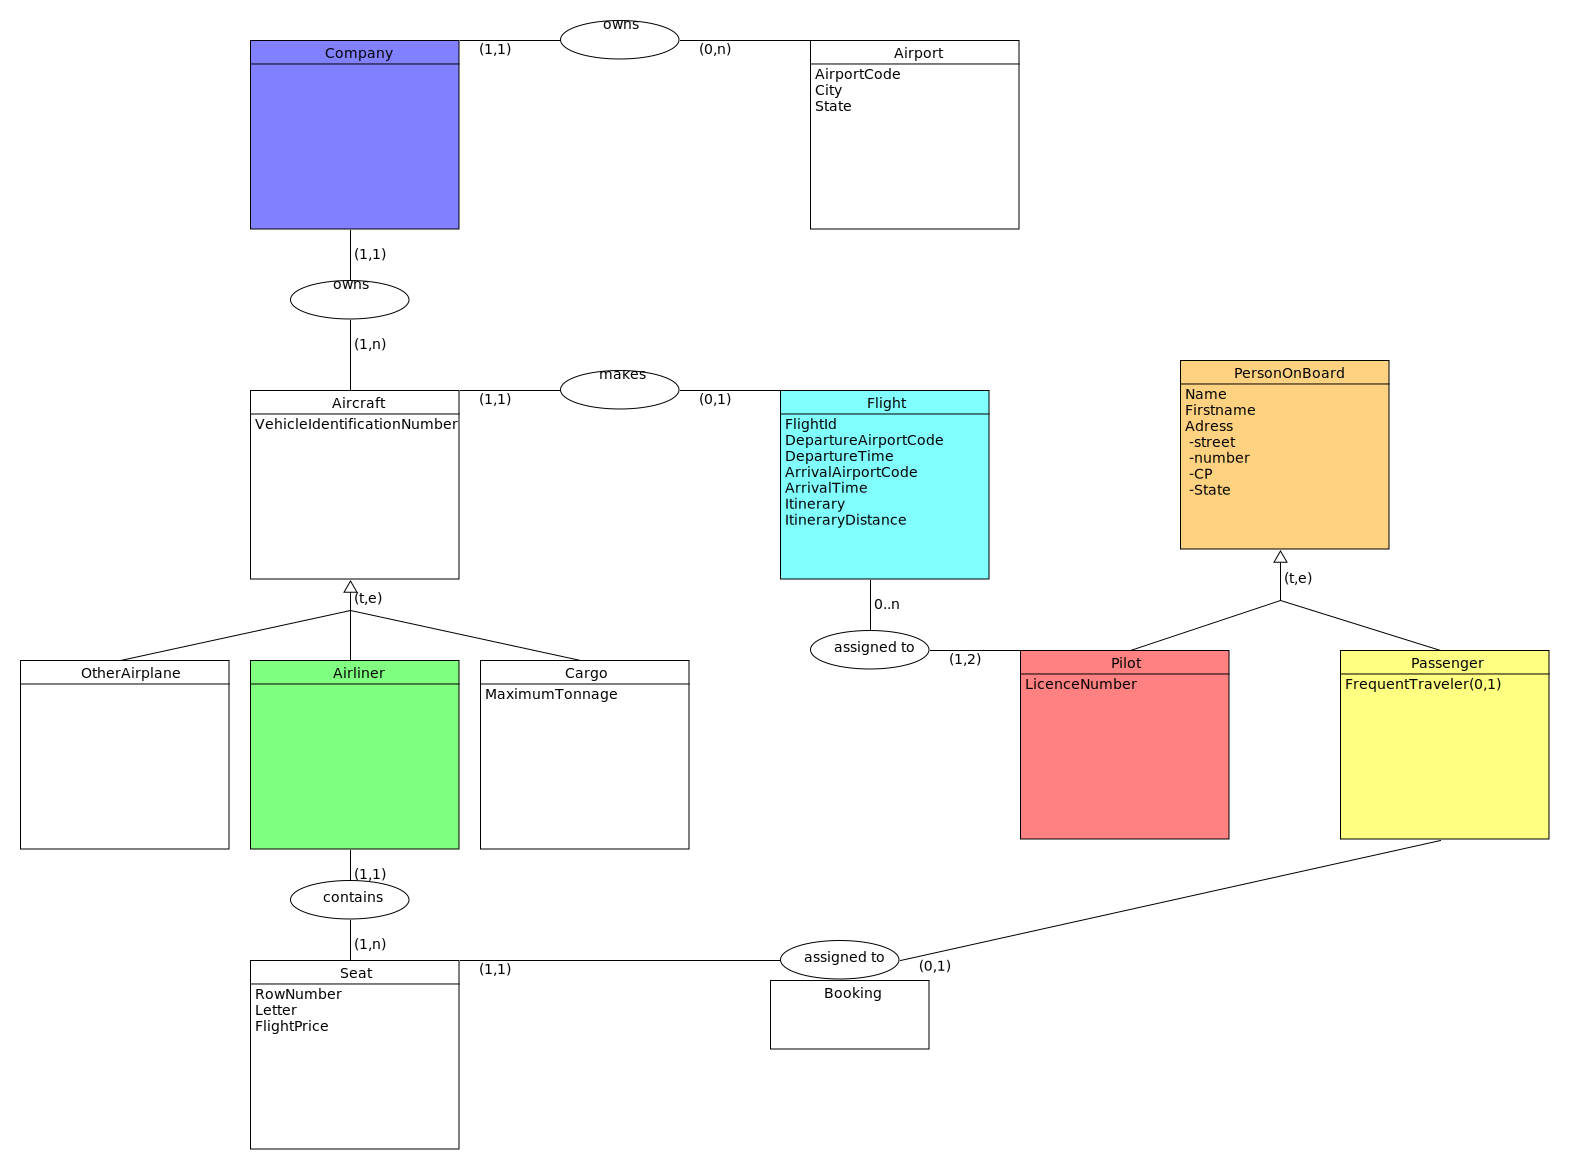
\includegraphics[width=\textwidth]{image/ATASCO-entity-relationship-diagram.png}
    \caption{Diagramme entité-association partie 1}
    \label{fig:diag_p1}
\end{figure}

% \MyIncludeGraphicsMaxSize{image/ATASCO-entity-relationship-diagram.png}[h]

\newpage
\subsection{Comparaison avec le modèle corrigé}
%\MyIncludeGraphicsMaxSize{image/correction.png}[h]
\begin{figure}[h]
    \centering
    \includegraphics[scale=0.6]{image/correction.png}
    \caption{Diagramme entité-association corrigé}
    \label{fig:diag_correction}
\end{figure}

\begin{itemize}
    \item meilleure lisibilité sur la figure \ref{fig:diag_p1}
    \item pas de table Etat dans la figure \ref{fig:diag_p1} donc, perte de précision et risque de confusion car si l'état est encodé sous forme de code chez le passager et sous son nom complet chez l'aéroport les deux ne seront pas égaux
    \item dans la figure \ref{fig:diag_correction} compagnie possède 0 à n avions (0 car cas extrême, moment de l'ajout dans database, nouvellement déclarée légalement, en faillite, transaction vente/rachat, etc.)
    \item "pilote operates" dans la figure \ref{fig:diag_p1} 0,1 vol faux, car le pilote peut être relié à plusieurs vols dans la database comme indiqué sur la figure \ref{fig:diag_correction} (0,n)
    \item un vol est opéré par un pilote et un copilote : cette possibilité est exclue par la figure \ref{fig:diag_correction}
    \item dans la figure \ref{fig:diag_p1} la clef du siège est composée de (aricraftid, row, number) alors que dans la figure \ref{fig:diag_correction} un id unique lui est attribué ce qui rend la manipulation des données plus facile.
    \item flight pourrait être une entité faible comme dans la figure  \ref{fig:diag_correction} car elle n'existe qu'à condition qu'elle soit reliée à un pilote
    \item réservation pourrait être une entité faible comme dans la figure \ref{fig:diag_correction} car elle n'existe qu'à condition qu'elle soit reliée à un avion
    \item seat pourrait être une entité faible comme dans la figure \ref{fig:diag_correction} car elle n'existe qu'à condition qu'elle soit reliée à un avion
    \item la relation P,e entre avion, avion de ligne et avions de fret dans la figure \ref{fig:diag_correction} permet de prendre en compte les avions de type autres alors que dans la figure \ref{fig:diag_p1}, seuls les avions de fret et de ligne étaient pris en compte
\end{itemize}


\newpage
\section{Traduction relationnelle}
\begin{itemize}
    \item Company(\underline{Id})
    \item Aircraft(\underline{Id},CompanyId, MaximumTonnage,NumberOfSeats)
    \subitem Aircraft.CompanyId ref Company.Id

    \item Airport(\underline{AirportCode},City,State)
    \item Flight(\underline{Id},AircraftId,StartAirport,EndAirport,ArrivalTime,DepartureTime,Distance)
    \subitem Flight.AircraftId ref Aircraft.Id
    \subitem Flight.StartAirport ref Airport.AirportCode
    \subitem Flight.EndAirport ref Airport.AirportCode

    \subitem Contrainte :
    \subsubitem - StartAiport doit être différent de EndAirport
    \subsubitem - DepartureTime (moment de départ) < ArrivalTime (moment d'arrivée)
    \subsubitem - Distance > 0

    \item Person(\underline{SSN}, FirstName,Name,AdressStreet,AdressNumber,AdressPC,AdressState,\underline{LicenseNumber},FrequentTraveller)

    \item FlightPilot(\underline{FlightId, PilotLicense})
    \subitem FlightPilot.FlightId ref Flight.Id
    \subitem FlightPilot.PilotLicense ref Person.LicenseNumber

    \item FlightPerson(\underline{FlightId, PersonId})
    \subitem FlightPerson.FlightId ref Flight.Id
    \subitem FlightPerson.PersonId ref Person.Id

    \item FlightTicket(\underline{PassengerSSN,FlightId},Price)
    \subitem FlightTicket.PassengerSSN ref Person.SSN
    \subitem FlightTicket.FlightId ref Flight.id

    \item Seat(\underline{AircraftId, Row, Number}, PassengerSSN)
    \subitem Seat.AircraftId ref Aircraft.Id
    \subitem Seat.PassengerSSN ref Person.Id

    \item SeatFlight(\underline{SeatRow, SeatNumber, FlightId})
    \subitem SeatFlight.SeatRow ref Seat.Row
    \subitem SeatFlight.SeatNumber ref Seat.Number
    \subitem SeatFlight.FlightId ref Flight.Id

\end{itemize}

\section{Justification}
Dans le tableau FLightPilot, LicenseNumber est une clé car il est unique pour chaque pilote. Un pilote est une personne, alors LicenseNumber est mis comme une clé secondaire dans le tableau Person.

\newline

Un vol est opéré par 2 pilotes, un capitaine et un copilote.
\newline
Beaucoup de requêtes n'ont pas de traduction en algèbre relationnel, calcul tuple car elles utilisent des fonctions qui ne sont pas (simplement) traduisible dans ce formalisme t.q. count, avg, window function, etc.
\newpage

\section{Requêtes}
\subsection{Requête 1}
\subsubsection{SQL}
\begin{verbatim}
select count(vol.id)
from vol,
     aviondefret
where vol.avionid = aviondefret.id;
\end{verbatim}

\newpage

\subsection{Requête 2}

\subsubsection{SQL}
\begin{verbatim}
select pilote.id
from pilote,
     réservation
where réservation.voyageurid = pilote.id;
\end{verbatim}
\subsubsection{Algèbre relationnel}
\[ \pi_{pilote.id}[\sigma_{reservation.voyageurid=pilote.id}(pilote, reservation)]\]
\subsubsection{Calcul tuple}
\[\{p.piloteid\; | \;pilote(p) \wedge \exists l(reservation(l) \wedge l.voyageurid=p.id )\}\]
\newpage
\subsection{Requête 3}
\subsubsection{SQL}
\begin{verbatim}
select *
from vol
where id = (
    select volleplusfrequenté.volid
    from (
             select count(voyageurid) as nombredepassager, réservation.volid
             from réservation
             group by réservation.volid
             order by nombredepassager desc
             limit 1
         ) as volleplusfrequenté
);
\end{verbatim}
\newpage

\subsection{Requête 4}
\subsubsection{SQL}
\begin{lstlisting}
select distinct vol.piloteid
from vol
except
select distinct vol.piloteid
from vol,
     aviondefret
where vol.avionid = aviondefret.id;
\end{lstlisting}
\subsubsection{Algèbre relationnel}
\[piloteslignes(piloteid) \xleftarrow{} \{\pi_{pilotedid} [\sigma_{avionid=aviondeligne.id}(vol, aviondeligne) - \sigma_{avionid=aviondefret.id}(vol, aviondefret)]\} \]
\subsubsection{Calcul tuple}
%\[\{\ v.piloteid\; | \;vol(v) \wedge  \exists a ( aviondeligne(a) \wedge v.avionid = a.id ) \wedge \lnot \exists f (aviondefret(f) \wedge  f.id = v.avionid) \}\]
\[\{\ p.piloteid\; | \;pilote(p) \wedge  \forall v\;vol(v) \xrightarrow{} ( p.id = v.piloteid \wedge \lnot \exists a(aviondefret(a) \wedge v.avionid = a.id)) \}\]
\newline
\newpage

\subsection{Requête 5}
\subsubsection{SQL}
\begin{verbatim}
select avg(distance), vol.heuredépart::date
from vol
where vol.avionid in (
    select avion.id
    from avion
    where avion.compagnieid in (
        select company.id
        from company
        where nom = 'ADVANCED AIR, LLC'
    )
)
group by vol.heuredépart::date
union
select avg(distance), vol.heuredépart::date
from vol
where vol.avionid in (
    select avion.id
    from avion
    where avion.compagnieid in (
        select company.id
        from company
        where nom = 'ABX Air Inc'
    )
)
group by vol.heuredépart::date;
\end{verbatim}
\newpage


\subsection{Requête 6}
\subsubsection{SQL}
\begin{verbatim}
select distinct aller.heurearrivee, retour.heuredepart
from vol as aller,
     vol as retour,
     aviondeligne
where aller.heuredepart::time > '07:00:00'
  and aller.heuredepart::date = retour.heuredepart::date
  and aller.heurearrivée::time < retour.heuredepart::time
  and retour.heuredepart >= aller.heurearrivée + '07:00:00'
  and aller.aeroportarriveecode = retour.aeroportdepartcode
  and aller.aeroportdepartcode = retour.aeroportarriveecode;
\end{verbatim}
\newpage

\subsection{Requête 7}
\subsubsection{SQL}
\begin{verbatim}
select avg(companyidpassager.nombredepassager), company.nom
from company
join(
    select avion.compagnieid, avionpassager.nombredepassager
    from avion
    join (
        select vol.avionid, passagervol.nombredepassager
        from vol
        join (
            select count(réservation.voyageurid) as nombredepassager, reservation.volid
            from réservation
            group by reservation.volid
            having count(reservation.voyageurid)<20
            ) as passagervol
        on passagervol.volid = vol.id
        ) as avionpassager
    on avion.id = avionpassager.avionid
    ) as companyidpassager
on company.id = companyidpassager.compagnieid
group by company.nom;
\end{verbatim}
\newpage

\subsection{Requête 8}
\subsubsection{SQL}
\begin{verbatim}
select volspilotes.piloteid, count(piloteid) as jourssconsecutifs
from (
         select vol.piloteid, -- listes des vols groupé par pilotes et leur dernier vol
                vol.heuredepart::date,
                vol.heurearrivée::date,
                lag(vol.heuredépart::date) -- départ du dernier vol
                over (partition by vol.piloteid order by vol.heuredépart)  as départderniervol,
                lag(vol.heurearrivée::date)
                over (partition by vol.piloteid order by vol.heurearrivée) as arrivéederniervol
         from vol) volspilotes
where volspilotes.heuredépart = volspilotes.départderniervol + interval '1 day'     -- vols consecutifs
   or volspilotes.heuredépart = volspilotes.arrivéederniervol + interval '1 day'    -- condition si le dernier vol s'étale sur deux jours
group by volspilotes.piloteid
order by jourssconsecutifs desc;
\end{verbatim}
\newpage

\subsection{Requête 9}
\subsubsection{SQL}

\begin{verbatim}
create table if not exists pilote_expert
(
    id        uuid primary key,
    date      date,
    estExpert boolean
);


create temp table temp_pilote_expert
(
    id_expert   varchar(128),
    date        varchar(128)
);

copy temp_pilote_expert (id_expert, date)
    from 'fichier.csv'
    delimiter ','
    header csv;


insert into pilote_expert(id, date, estExpert)
select split_part(temp_pilote_expert.id_expert, '--', 2)::uuid,
       temp_pilote_expert.date::timestamp,
       case -- switch comme en C++
           when split_part(temp_pilote_expert.id_expert, '--', 1) = 'existing-expert' then true
           when split_part(temp_pilote_expert.id_expert, '--', 1) = 'new-expert' then false
           else false
           end
from temp_pilote_expert
where not exists( -- verification que l'on n'insere pas une ligne deja presenten
        select pilote_expert.id
        from pilote_expert
        where id = split_part(temp_pilote_expert.id_expert, '--', 2)::uuid
    );

\end{verbatim}
\newpage

\subsection{Requête 10}
\subsubsection{SQL}

%\begin{lstlisting}[language=SQL]
\begin{verbatim}

CREATE EXTENSION IF NOT EXISTS "uuid-ossp";


create table if not exists aeroportsujets
(
    id    uuid primary key,
    code  varchar(8),
    sujet text
);


insert into aeroportsujets(id, code, sujet)
    (
        select uuid_generate_v1(), 'AKN', 'mobilité'
    );


create table if not exists discussion
(
    id         uuid primary key,
    message    text,
    expediteur varchar(8)
);

\end{verbatim}

\section{Référence} \label{sec:ref}

\begin{itemize}
    \item Wikipédia modèle entité-association "\url{https://fr.wikipedia.org/wiki/Mod%C3%A8le_entit%C3%A9-association}" vu le 05/05/2022
\end{itemize}

\end{document}
